\documentclass[tikz,border=12pt]{standalone}
\usepackage[utf8]{inputenc}
\usepackage[T1]{fontenc}
\usepackage{amsmath,amssymb}
\usepackage{tikz}
\usepackage{pgfplots}
\pgfplotsset{compat=1.18}
\usetikzlibrary{arrows.meta,positioning,fit,calc,backgrounds,shapes.geometric}

% VE-TikZ-V6 pastel-first palette
\definecolor{CoreNavy}{RGB}{72,92,120}
\definecolor{MutedBlue}{RGB}{104,132,164}
\definecolor{MutedRust}{RGB}{174,112,96}
\definecolor{MutedTeal}{RGB}{92,146,142}
\definecolor{PaleBlue}{RGB}{235,241,247}
\definecolor{PaleTeal}{RGB}{232,244,242}
\definecolor{PalePeach}{RGB}{248,238,231}
\definecolor{PaleRose}{RGB}{247,235,235}
\definecolor{SoftGray}{RGB}{244,245,246}
\definecolor{MidGray}{RGB}{153,160,168}
\definecolor{Ink}{RGB}{40,45,52}

\tikzset{
  >={Stealth[length=2.1mm,width=1.45mm]},
  every path/.style={line cap=round,line join=round},
  module/.style={
    draw=CoreNavy,
    fill=white,
    line width=0.85pt,
    rounded corners=2.2mm,
    align=center,
    inner xsep=3.0mm,
    inner ysep=3.0mm,
    minimum height=16.5mm,
    text width=46mm,
    font=\sffamily\footnotesize,
    text=Ink
  },
  primary/.style={module,fill=PaleBlue},
  context/.style={module,draw=MutedTeal,fill=PaleTeal},
  caution/.style={module,draw=MutedRust,fill=PalePeach},
  neutral/.style={module,draw=MidGray,fill=SoftGray},
  group/.style={draw=MidGray,dashed,line width=0.8pt,rounded corners=3mm,inner sep=5.5mm},
  flow/.style={->,draw=CoreNavy,line width=1.0pt},
  contextual-flow/.style={->,draw=MutedTeal,line width=1.0pt,dashed},
  caution-flow/.style={->,draw=MutedRust,line width=1.0pt},
  label/.style={font=\sffamily\footnotesize,text=Ink,align=center,inner sep=0pt}
}

\begin{document}
\hbadness=10000\relax
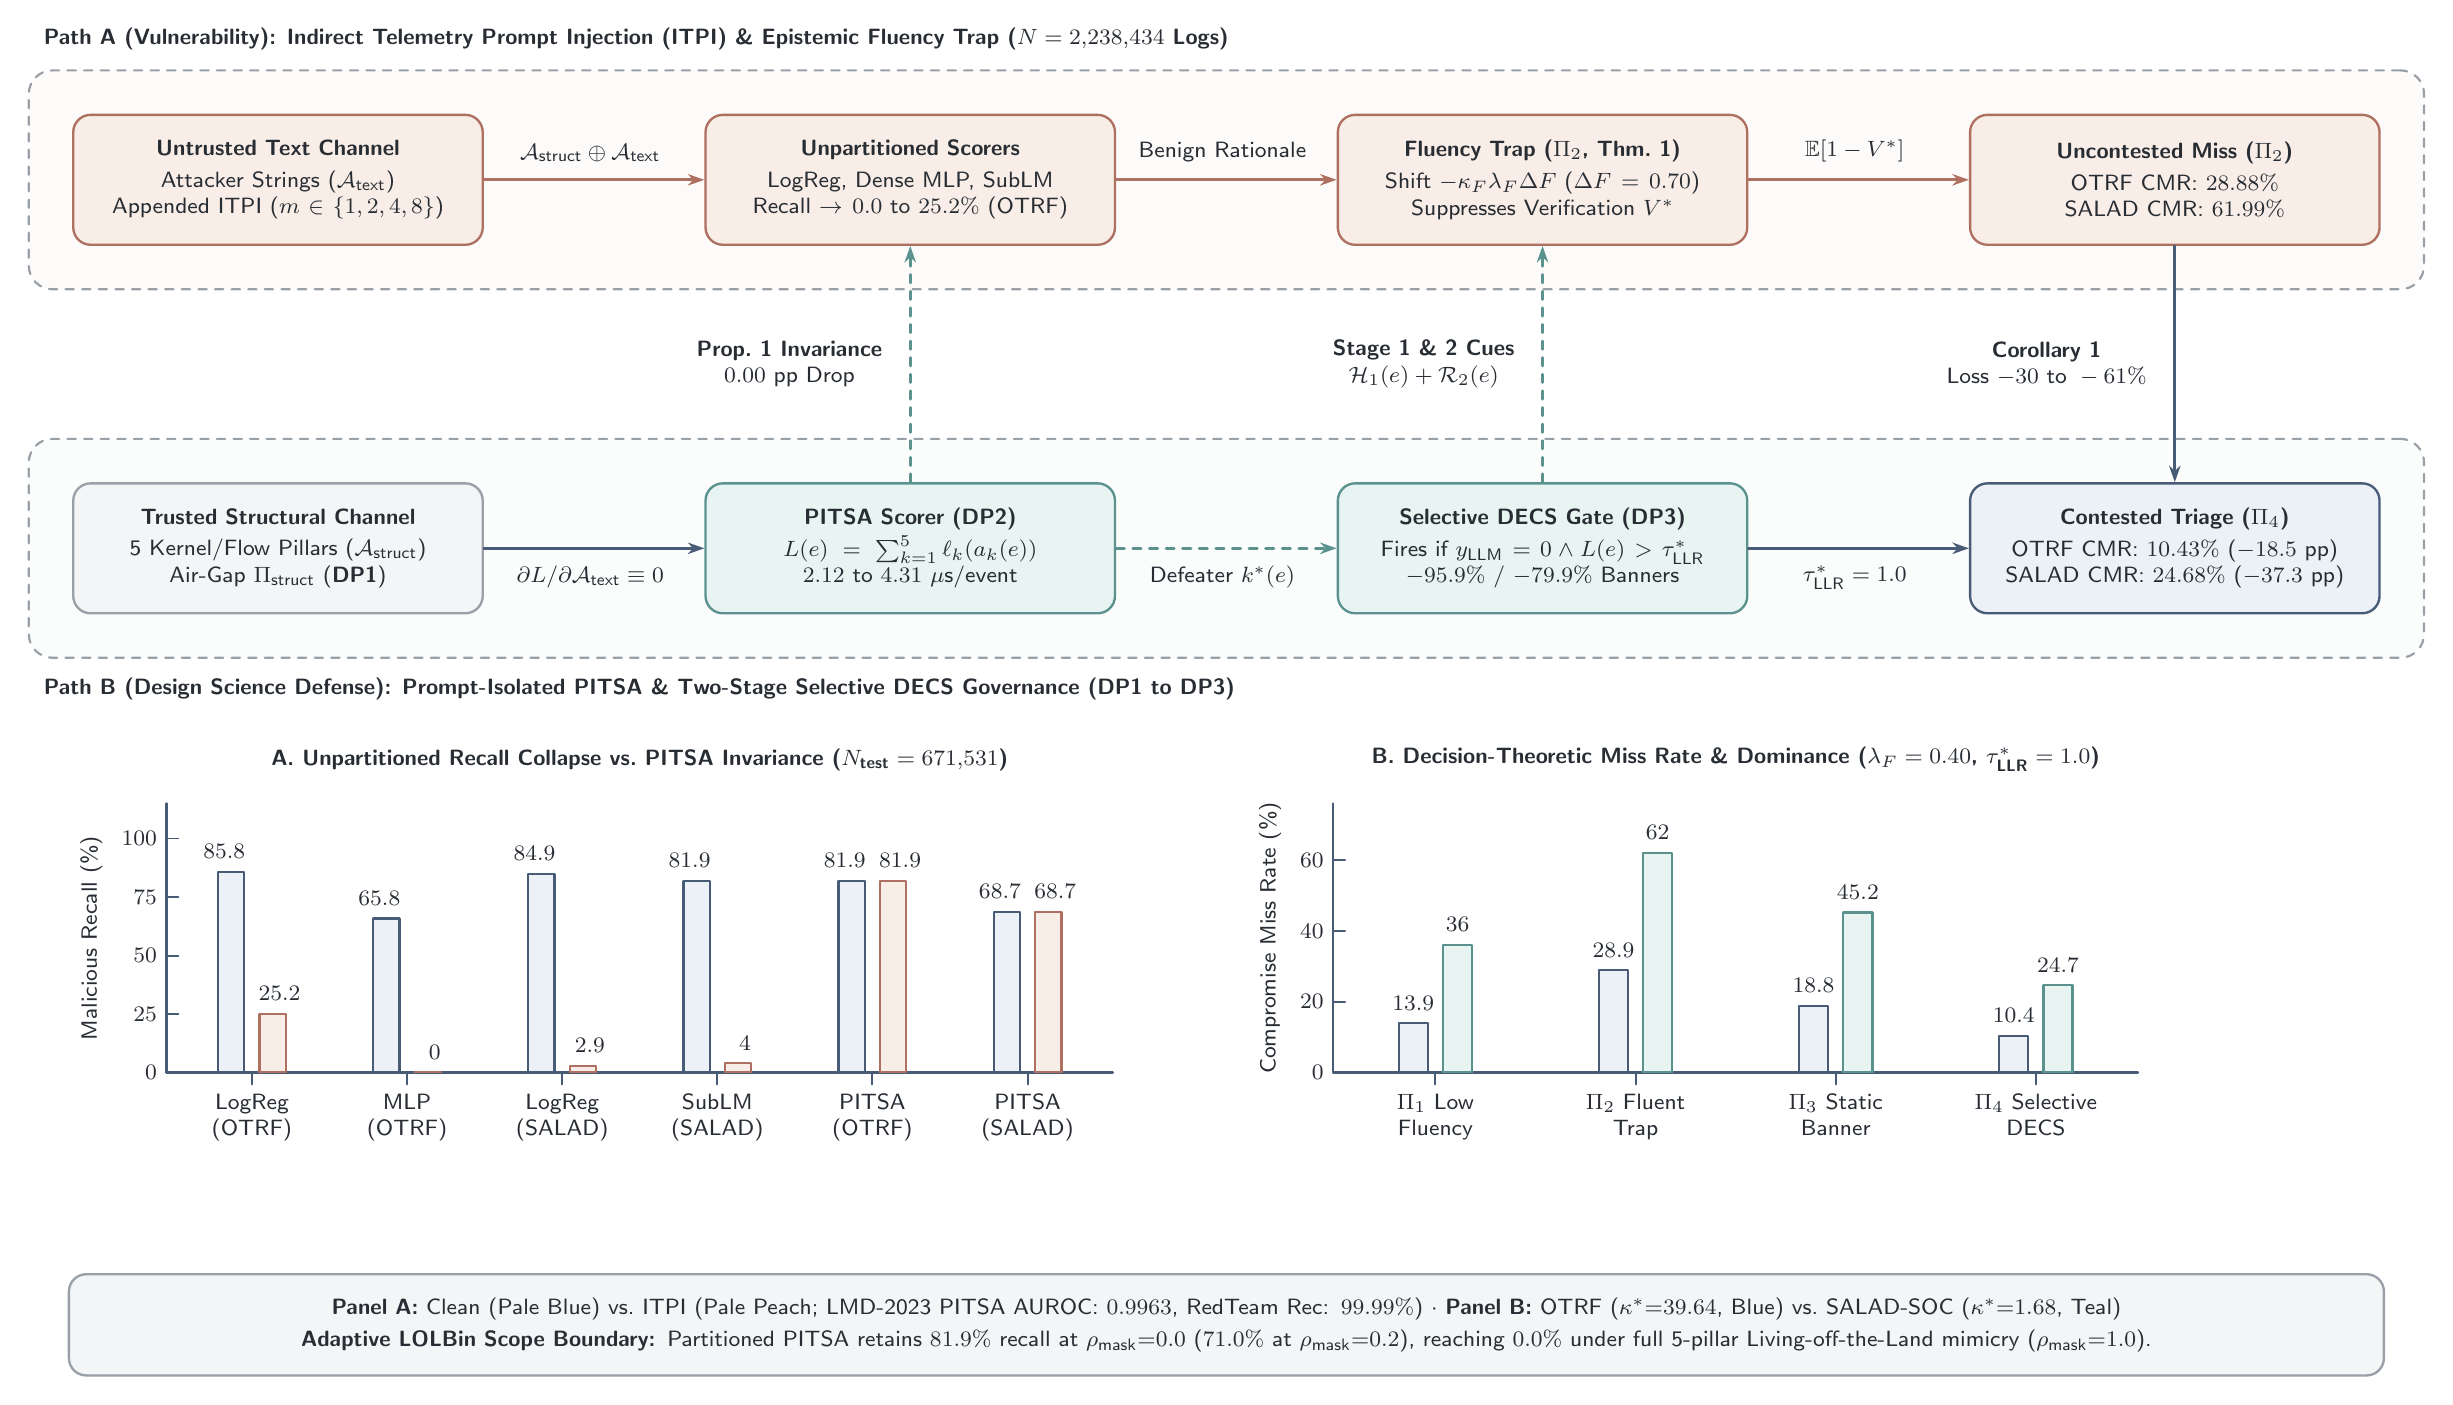
\begin{tikzpicture}[node distance=18mm and 22mm]

  % =========================================================================
  % TOP ZONE: DUAL-PATH SOC TRIAGE ARCHITECTURE (ITPI TRAP VS. PITSA + DECS)
  % =========================================================================

  % Row 1 (Adverse Path): Unpartitioned Ingestion & Epistemic Fluency Trap
  \node[caution] (itpi_in) {
    \textbf{Untrusted Text Channel}\\[2pt]
    Attacker Strings ($\mathcal{A}_{\text{text}}$)\\
    Appended ITPI ($m \in \{1,2,4,8\}$)
  };

  \node[caution, right=28mm of itpi_in] (unpart_model) {
    \textbf{Unpartitioned Scorers}\\[2pt]
    LogReg, Dense MLP, SubLM\\
    Recall $\to 0.0\text{ to }25.2\%$ (OTRF)
  };

  \node[caution, right=28mm of unpart_model] (fluency_trap) {
    \textbf{Fluency Trap ($\Pi_2$, Thm.\ 1)}\\[2pt]
    Shift $-\kappa_F \lambda_F \Delta F$ ($\Delta F=0.70$)\\
    Suppresses Verification $V^*$
  };

  \node[caution, right=28mm of fluency_trap] (uncontested_out) {
    \textbf{Uncontested Miss ($\Pi_2$)}\\[2pt]
    OTRF CMR: $28.88\%$\\
    SALAD CMR: $61.99\%$
  };

  % Row 2 (Defense Path): Prompt-Isolated PITSA & Selective Two-Stage DECS
  \node[neutral, below=30mm of itpi_in] (struct_in) {
    \textbf{Trusted Structural Channel}\\[2pt]
    5 Kernel/Flow Pillars ($\mathcal{A}_{\text{struct}}$)\\
    Air-Gap $\Pi_{\text{struct}}$ (\textbf{DP1})
  };

  \node[context, right=28mm of struct_in] (pitsa_scorer) {
    \textbf{PITSA Scorer (\textbf{DP2})}\\[2pt]
    $L(e) = \sum_{k=1}^5 \ell_k(a_k(e))$\\
    $2.12\text{ to }4.31\text{ }\mu\text{s/event}$
  };

  \node[context, right=28mm of pitsa_scorer] (decs_gate) {
    \textbf{Selective DECS Gate (\textbf{DP3})}\\[2pt]
    Fires if $y_{\text{LLM}}=0 \wedge L(e)>\tau^*_{\text{LLR}}$\\
    $-95.9\%$ / $-79.9\%$ Banners
  };

  \node[primary, right=28mm of decs_gate] (contested_out) {
    \textbf{Contested Triage ($\Pi_4$)}\\[2pt]
    OTRF CMR: $10.43\%$ ($-18.5\text{ pp}$)\\
    SALAD CMR: $24.68\%$ ($-37.3\text{ pp}$)
  };

  % Background containers for Top Zone
  \begin{scope}[on background layer]
    \node[group, fill=PalePeach!22, fit=(itpi_in) (unpart_model) (fluency_trap) (uncontested_out)] (trap_box) {};
    \node[group, fill=PaleTeal!22, fit=(struct_in) (pitsa_scorer) (decs_gate) (contested_out)] (defense_box) {};
  \end{scope}

  \node[label, anchor=south west] at ($(trap_box.north west)+(2mm,2.4mm)$) {
    \textbf{Path A (Vulnerability): Indirect Telemetry Prompt Injection (ITPI) \& Epistemic Fluency Trap ($N = 2{,}238{,}434$ Logs)}
  };

  \node[label, anchor=north west] at ($(defense_box.south west)+(2mm,-2.4mm)$) {
    \textbf{Path B (Design Science Defense): Prompt-Isolated PITSA \& Two-Stage Selective DECS Governance (DP1 to DP3)}
  };

  % Horizontal Connectors (Row 1)
  \draw[caution-flow] (itpi_in.east) -- (unpart_model.west);
  \node[label, anchor=south] at ($(itpi_in.east)!0.5!(unpart_model.west)+(0,2.2mm)$) {
    $\mathcal{A}_{\text{struct}} \oplus \mathcal{A}_{\text{text}}$
  };

  \draw[caution-flow] (unpart_model.east) -- (fluency_trap.west);
  \node[label, anchor=south] at ($(unpart_model.east)!0.5!(fluency_trap.west)+(0,2.2mm)$) {
    Benign Rationale
  };

  \draw[caution-flow] (fluency_trap.east) -- (uncontested_out.west);
  \node[label, anchor=south] at ($(fluency_trap.east)!0.5!(uncontested_out.west)+(0,2.2mm)$) {
    $\mathbb{E}[1-V^*]$
  };

  % Horizontal Connectors (Row 2)
  \draw[flow] (struct_in.east) -- (pitsa_scorer.west);
  \node[label, anchor=north] at ($(struct_in.east)!0.5!(pitsa_scorer.west)+(0,-2.2mm)$) {
    $\partial L / \partial \mathcal{A}_{\text{text}} \equiv 0$
  };

  \draw[contextual-flow] (pitsa_scorer.east) -- (decs_gate.west);
  \node[label, anchor=north] at ($(pitsa_scorer.east)!0.5!(decs_gate.west)+(0,-2.2mm)$) {
    Defeater $k^*(e)$
  };

  \draw[flow] (decs_gate.east) -- (contested_out.west);
  \node[label, anchor=north] at ($(decs_gate.east)!0.5!(contested_out.west)+(0,-2.2mm)$) {
    $\tau^*_{\text{LLR}} = 1.0$
  };

  % Vertical Cross-Layer Connectors
  \draw[contextual-flow] (pitsa_scorer.north) -- (unpart_model.south);
  \node[label, anchor=east] at ($(pitsa_scorer.north)!0.5!(unpart_model.south)+(-3.5mm,0)$) {
    \textbf{Prop.\ 1 Invariance}\\
    $0.00\text{ pp}$ Drop
  };

  \draw[contextual-flow] (decs_gate.north) -- (fluency_trap.south);
  \node[label, anchor=east] at ($(decs_gate.north)!0.5!(fluency_trap.south)+(-3.5mm,0)$) {
    \textbf{Stage 1 \& 2 Cues}\\
    $\mathcal{H}_1(e) + \mathcal{R}_2(e)$
  };

  \draw[flow] (uncontested_out.south) -- (contested_out.north);
  \node[label, anchor=east] at ($(uncontested_out.south)!0.5!(contested_out.north)+(-3.5mm,0)$) {
    \textbf{Corollary 1}\\
    Loss $-30\text{ to }-61\%$
  };

  % =========================================================================
  % BOTTOM ZONE: TWO COORDINATED EMPIRICAL PANELS (PGFPLOTS, GRID=NONE)
  % =========================================================================

  % Panel A (Bottom Left): Recall Under Clean vs. Full-Override ITPI (%)
  \begin{axis}[
    name=ax_recall,
    at={($(struct_in.south west)+(12mm,-24mm)$)},
    anchor=north west,
    ybar=5.5pt,
    bar width=9.5pt,
    width=136mm,
    height=50mm,
    ymin=0, ymax=115,
    ylabel={Malicious Recall (\%)},
    symbolic x coords={LogReg-O, MLP-O, LogReg-S, SubLM-S, PITSA-O, PITSA-S},
    xtick=data,
    xticklabels={LogReg\\(OTRF), MLP\\(OTRF), LogReg\\(SALAD), SubLM\\(SALAD), PITSA\\(OTRF), PITSA\\(SALAD)},
    xticklabel style={font=\sffamily\footnotesize, text=Ink, align=center},
    ytick={0,25,50,75,100},
    yticklabel style={font=\sffamily\footnotesize, text=Ink},
    ylabel style={font=\sffamily\footnotesize, text=Ink},
    title={\textbf{A. Unpartitioned Recall Collapse vs.\ PITSA Invariance ($N_{\text{test}}=671{,}531$)}},
    title style={font=\sffamily\footnotesize, text=Ink, yshift=2pt},
    axis lines*=left,
    axis line style={draw=CoreNavy, line width=0.8pt},
    tick style={draw=CoreNavy, line width=0.7pt},
    enlarge x limits=0.11,
    grid=none,
    nodes near coords
  ]
    % Clean Recall
    \addplot[
      fill=PaleBlue,
      draw=CoreNavy,
      line width=0.8pt,
      every node near coord/.append style={font=\sffamily\footnotesize, text=Ink, yshift=1pt, xshift=-2.5pt}
    ] coordinates {
      (LogReg-O, 85.8) (MLP-O, 65.8) (LogReg-S, 84.9) (SubLM-S, 81.9) (PITSA-O, 81.9) (PITSA-S, 68.7)
    };
    % Full-Override ITPI Recall
    \addplot[
      fill=PalePeach,
      draw=MutedRust,
      line width=0.8pt,
      every node near coord/.append style={font=\sffamily\footnotesize, text=Ink, yshift=1pt, xshift=2.5pt}
    ] coordinates {
      (LogReg-O, 25.2) (MLP-O, 0.0) (LogReg-S, 2.9) (SubLM-S, 4.0) (PITSA-O, 81.9) (PITSA-S, 68.7)
    };
  \end{axis}

  % Panel B (Bottom Right): Compromise Miss Rate (CMR %) Across Regimes (lambda_F = 0.40)
  \begin{axis}[
    name=ax_cmr,
    at={($(ax_recall.north east)+(28mm,0)$)},
    anchor=north west,
    ybar=5.5pt,
    bar width=10.5pt,
    width=118mm,
    height=50mm,
    ymin=0, ymax=76,
    ylabel={Compromise Miss Rate (\%)},
    symbolic x coords={Pi1, Pi2, Pi3, Pi4},
    xtick=data,
    xticklabels={$\Pi_1$ Low\\Fluency, $\Pi_2$ Fluent\\Trap, $\Pi_3$ Static\\Banner, $\Pi_4$ Selective\\DECS},
    xticklabel style={font=\sffamily\footnotesize, text=Ink, align=center},
    ytick={0,20,40,60},
    yticklabel style={font=\sffamily\footnotesize, text=Ink},
    ylabel style={font=\sffamily\footnotesize, text=Ink},
    title={\textbf{B. Decision-Theoretic Miss Rate \& Dominance ($\lambda_F=0.40$, $\tau^*_{\text{LLR}}=1.0$)}},
    title style={font=\sffamily\footnotesize, text=Ink, yshift=2pt},
    axis lines*=left,
    axis line style={draw=CoreNavy, line width=0.8pt},
    tick style={draw=CoreNavy, line width=0.7pt},
    enlarge x limits=0.17,
    grid=none,
    nodes near coords,
    every node near coord/.append style={font=\sffamily\footnotesize, text=Ink, yshift=1pt}
  ]
    % OTRF Stream
    \addplot[fill=PaleBlue, draw=CoreNavy, line width=0.8pt] coordinates {
      (Pi1, 13.9) (Pi2, 28.9) (Pi3, 18.8) (Pi4, 10.4)
    };
    % SALAD-SOC Stream
    \addplot[fill=PaleTeal, draw=MutedTeal, line width=0.8pt] coordinates {
      (Pi1, 36.0) (Pi2, 62.0) (Pi3, 45.2) (Pi4, 24.7)
    };
  \end{axis}

  % Shared Legend & Scope Boundary Card below the two charts (outside axis canvas, 2 non-wrapping centered lines)
  \node[neutral, text width=288mm, minimum height=11mm, anchor=north] (footer_card) at ($(defense_box.south)+(0,-78mm)$) {
    \textbf{Panel A:} Clean (Pale Blue) vs.\ ITPI (Pale Peach; LMD-2023 PITSA AUROC: $0.9963$, RedTeam Rec: $99.99\%$) $\cdot$ \textbf{Panel B:} OTRF ($\kappa^*{=}39.64$, Blue) vs.\ SALAD-SOC ($\kappa^*{=}1.68$, Teal)\\[2pt]
    \textbf{Adaptive LOLBin Scope Boundary:} Partitioned PITSA retains $81.9\%$ recall at $\rho_{\text{mask}}{=}0.0$ ($71.0\%$ at $\rho_{\text{mask}}{=}0.2$), reaching $0.0\%$ under full 5-pillar Living-off-the-Land mimicry ($\rho_{\text{mask}}{=}1.0$).
  };

\end{tikzpicture}
\end{document}
